\documentclass[12pt]{article}
%%%%%%%%%%%%%%%%%%%%%%%%%%%%%%%%%%%%%%%%%
\usepackage{amscd}\usepackage{amsmath}\usepackage{amssymb}\usepackage{graphicx}
\usepackage{amsthm}\usepackage{latexsym}\usepackage{verbatim}\usepackage{multicol}
\setlength{\textheight}{8.5in} \setlength{\topmargin}{0.in}
\setlength{\headheight}{0.0in} \setlength{\headsep}{0.0in}
\setlength{\leftmargin}{0.5in}\setlength{\oddsidemargin}{0.0in}
%\setlength{\parindent}{1pc}\linespread{1.6}
\setlength{\textwidth}{6.7in}
\newcommand{\noi}{\noindent}
\newenvironment{loose_item}{
\begin{itemize}
  \setlength{\itemsep}{75pt}
  \setlength{\parskip}{40pt}
  \setlength{\parsep}{40pt}
}{\end{itemize}}
%%%%%%%%%%%%%%%%%%%%%%%%%%%%%%%%%%%%%%%%%
\begin{document}

\begin{center}
Math 4B Midterm Review Problems

October 30, 2014
  
\end{center}

\noindent These are practice problems to help you prepare for your midterm, you do not need to turn in solutions.  You should think of this as a starting point for organizing your study plan.   You should also review your DPs, old homework problems and problems from the lecture slides.
\vskip 2mm
\noi Your midterm will cover material from sections 1.1, 1.2, 2.1-2.5, 2.9, 3.1-3.4 and 3.7  
\begin{enumerate}


\item The slope field below corresponds to a linear DE of the form
$$y' + p(t)y = g(t)$$
\begin{center}
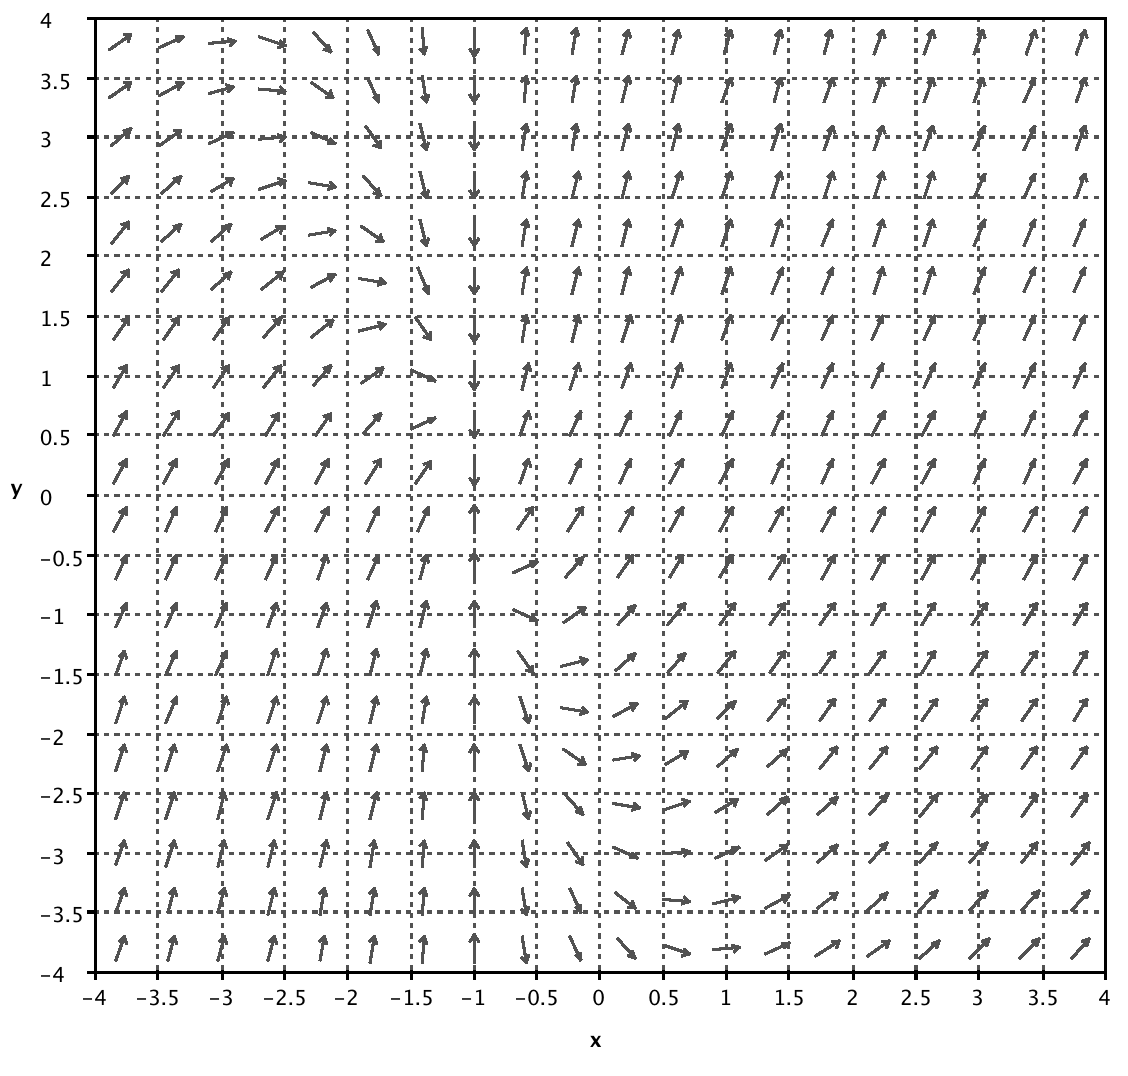
\includegraphics[width=80mm]{slope.png}
\end{center}
\begin{itemize}
\item[(a)] Is the corresponding DE is autonomous?  How can you tell?
\item[(b)] Sketch the solution curve corresponding to the initial condition $y(0) = 1$.  What is the largest interval in which this solution of the IVP can exist?  How can you tell? 
\item[(c)] Describe the long term behavior of your solution from part (b).
\item[(d)] Sketch the solution curve corresponding to the initial condition $y(-2) = 1$. What is the largest interval in which this solution of the IVP can exist?  How can you tell? 
\item[(e)] Describe the long term behavior of your solution from part (d).

\end{itemize}

%%%%%%%%

\item Which of the following differential equations are separable?
Circle \textit{all} that apply.
\begin{multicols}{2}
\begin{itemize}
\item[(A)] $y' + y^2\sin x = 0$
\item[(B)] $y' = \dfrac{3y^2-x^2}{2xy}$
\item[(C)] $y' = \dfrac{x(x^2 + 1)}{4y^3}$
\item[(D)] $\dfrac{dr}{d\theta} = \dfrac{r^2}{\theta}$
\end{itemize}
\end{multicols}

%%%%%


\item Consider the following \textit{autonomous differential equation}:
$$y' = f(y)$$
Which of the following statements are true?
Circle \textit{all} that apply and justify your choices.
\begin{itemize}
\item[(A)] We can find the values of $y$ that give equilibrium solutions to the DE by solving the equation $f(y)=0$.
\item[(B)] The corresponding IVP with any initial conditions will have unique solutions.
\item[(C)] The equation is separable.
\item[(D)] The slope field for such an equation will have horizontal isoclines.
\end{itemize}

%%%%%


\item A deposit into a savings account earns interest, which is just a fraction of your deposit added to the total at regular intervals.  
\begin{itemize}
\item[(a)] Suppose your account earns $8\%$ each year and that interest is compounded once a year, i.e. $8\%$ of the amount is added each year.  How much money will you have after 5 years with an initial deposit of \$$100$?   After $N$ years?
\item[(b)] Now suppose the interest is compounded monthly.  How much will you have in the account after 5 years?
\item[(c)] Write down a \textit{difference equation} that describes how the account value is changing.  Suppose the annual interest rate $r$ is compounded $n$ times per year.  Your difference equation should look something like
$$A_{k+1} - A_k = ??$$
\item[(d)] Now suppose the bank makes it's payments more and more often:  daily, hourly, every minute, every second... continuously.  What will your difference equation look like if interest is compounded continuously?  HINT: Let $A(t) = A_k$ and let $\Delta t = \frac{1}{n}$, then find an expression for $\Delta A = A(t+\Delta t) - A(t)$.  In the limit as $\Delta t \to 0$, you should get a \textit{differential equation}.
\item[(e)] Compare the return after 5 years on two accounts with $A_0 = \$100$ and $r = 8\%$ - one compounded monthly and one compounded continuously.  What kind of account do you want to invest in?
\end{itemize}

%%%%%%%%%%%%%%%


\item Sketch slope fields along with three solution curves for the following IVPs.  Indicate an initial condition that corresponds to each of your solution curves.
\begin{multicols}{3}
\begin{itemize}
\item[(a)] $y' + 3y = t$
\item[(b)] $y' = y(y+1)$
\item[(c)] $y' = 2t+y$
\end{itemize}
\end{multicols}

\newpage

\item Consider the separable equation:
$$y' = \frac{x^2}{(1-y^2)}$$
Explain how to use separation of variables to solve this DE.  Be sure to explain all steps carefully - including how you jump from integrating the LHS `$dx$' to integrating `$dy$'.  
\\


\item Newton's Law of Cooling states that an object will cool down (or heat up) at a rate proportional to the difference between the temperature of the object and the ambient temperature.  
\begin{itemize}
\item[(a)] Write a differential equation that models the rate a cup of coffee will cool down.  Let $k$ be the constant of proportionality, $y(t)$ the temperature of the coffee and $T$ the ambient temperature.
\item[(b)] Now suppose suppose the cup of coffee is made with boiling hot water and set in a room where the temperature is $20^{\circ}$C and the coffee cools to $90^{\circ}$C in 2 minutes.  How long will it take the coffee to cool $60^{\circ}$C?
\end{itemize}



\item A ball is project vertically upwards in viscous fluid (think honey).  The (force due to the) viscosity of the fluid acts to slow the motion of the object at a rate proportional to it's speed (let $k$ be the constant of proportionality).  Assume that the gravitational force acting on the ball is $mg$ where $m= 1$kg is the mass of the ball and $g\approx 10$m/s$^2$ is a good-enough estimate of acceleration due to gravity.
\begin{itemize}
\item[(a)] Let $v(t)$ be the velocity of the ball at time $t$.  Use Newton's Law to write a differential equation that models the situation.  
\item[(b)] Find the velocity $v(t)$ of the ball at any time $t$ if the ball's initial velocity is $v_0 = 5m/s$.
\item[(c)] Describe the behavior of $v(t)$ as $t\to \infty$.  What does this indicate about the motion of the ball?
\end{itemize}



\item Solve the IVPs and then determine where the solution is defined.
\begin{multicols}{2}
\begin{itemize}
\item[(a)] $\dfrac{dr}{d\theta} = \dfrac{r^2}{\theta}, \ \ r(1)=2$
\item[(b)] $y' = (1-2x)y^2, \ \ y(0) = -1/6.$
\item[(c)] $y' = \dfrac{x(x^2 + 1)}{4y^3}, \ \ y(0) = -1/\sqrt{2}.$
\end{itemize}
\end{multicols}



\item Solve the following linear DEs and describe how solutions behave as $t\to \infty$.  
\begin{multicols}{3}
\begin{itemize}
\item[(a)] $y' + \dfrac{y}{t} = \cos (t)$
\item[(b)] $2y' + y = 3t$
\item[(c)] $ty' -y = t^2e^{-t}$
\end{itemize}
\end{multicols}

\item Consider the linear DE with initial conditions:
$$\ln(t)y' + y = \cot(t),\ \  y(2) = 3.$$
Use the E/U Theorem for Linear DEs to determine the largest interval where we have a unique solution to the IVP.


\item Let's explore existence and uniqueness for linear equations.  For the following equations, determine where the Existence and Uniqueness Theorem for Linear DEs holds.  Then see if you can piece together a continuous solution to the IVP defined for all $t \geq 0$ anyways.
\begin{itemize}
\item[(a)] $y' + 2y = g(t), \ \ y(0) = 0$, where 
$$g(t) = \left\{ \begin{array}{lcr} 1 &\text{if}& 0\leq t < 1\\ 0 & \text{if} & t>1\end{array}\right.$$

\item[(b)] $y' + p(t)y = 0, \ y(0) = 1$, where
$$p(t) = \left\{ \begin{array}{lcr} 2 &\text{if}& 0\leq t < 1\\ 1 & \text{if} & t>1\end{array}\right.$$
\end{itemize}



\item Make a substitution to solve the following DEs.  
\begin{itemize}
\item[(a)] $y' = \dfrac{3y^2-x^2}{2xy}$, let $v= \frac{y}{x}$.
\item[(b)] $y' + 1 = (y+x)^2$, let $v = x+y$.
\item[(c)] $2yy' = \cos(y^2)$, let $v = y^2$.
\end{itemize}


\item Consider the following autonomous DE:
$$ y' = y^2(4-y^2).$$
Use qualitative information to sketch solution curves to this equation:
\begin{itemize}
\item[(a)] Find the equilibrium solutions and classify them as stable, semistable or unstable.
\item[(b)] Find a formula for $y''$ and use this to determine the concavity of solutions for certain values of $y$.
\item[(c)] Sketch several graphs of solutions in the $ty$-plane.
\end{itemize}

\item An object on a table attached to a spring and wall (as pictured below) is pulled to the right, stretching the spring, and released.  The same object is then pulled twice as far and released.  What is the relationship between the two simple harmonic motions?  Will the period of the second be twice that of the first?  What about the amplitudes?

\begin{center}
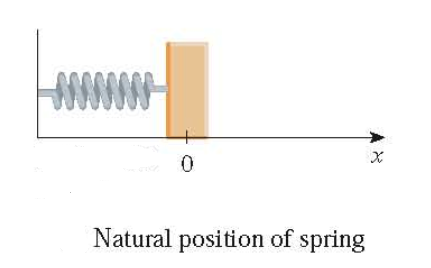
\includegraphics[width= 50mm]{spring1.png}
\end{center}


 
 \item A block with mass 1 kg stretches a spring 4.9 m when it is attached.  The mass is a attached to a viscous damper with a damping constant of $b$ Ns/m.  
\begin{itemize} 
\item[(a)] For which value(s) of $b$ is the system critically damped? Overdamped? Underdamped? Undamped?
\item[(b)] Suppose $b=3$.  If the mass is set in motion from its equilibrium position with downward velocity of 2m/s, find its position $x$ at any time $t$.
\item[(c)] Show that your solution for part (b) can only cross the $x$-axis once (if at all).
\end{itemize}

\item (a) Verify that the functions $y_1(x) = -\dfrac{1}{x}$ and $y_2(x) = -\dfrac{1}{x+2}$ are solutions to the differential equation
\begin{equation}
\label{nonlin}
y'' - 2y^3 = 0.
\end{equation}

\noi (b) Verify that an arbitrary linear combination of $y_1$ and $y_2$ is \textbf{not} a solution to the differential equation (\ref{nonlin}).

\noi(c) It seems that this equation doesn't satisfy the principle of superposition from section 3.2 of your textbook.  Explain why not.\\



\item Consider the IVP $t^2y'' - t(t+2)y' + (t+2)y = 0$, $y(1)=a$, $y'(1)=b$
\begin{itemize}
\item[(a)] Verify that $y_1(t) = t$ is a solution to the DE.  For which values of $a$ and $b$ is the solution to the IVP a scalar multiple of $y_1$?
\item[(b)] Explain how you know that the fundamental set for this DE will have at least one other solution.  Use Theorem 3.2.1 from your book in your argument.
\item[(c)] Use reduction of order to find the second solution for the fundamental set for this DE.
\item[(d)] Solve the IVP for $a = 1$ and $b=0$.
\end{itemize}



\item Consider the IVP $y''-2y'+2y = 0$, $y(0) = 2$ and $y'(0) = 0$.  
\begin{itemize}
\item[(a)] Find a fundamental set of \textit{complex} solutions to the DE.  Then find a solution to the IVP from among those complex solutions.
\item[(b)] Use Euler's Formula to find a fundamental set of \textit{real} solutions to the DE.
\item[(c)] Find a solution to the IVP from among your real solutions.  Then use Euler's formula to show that this solution is the same as the solution you found in part (a).
\end{itemize}



\end{enumerate}


%%%%%%%%%%%%%%%%%%%%%%%%%%%%%%%%%%%%%%%%%
\end{document}
\item Consider a first order IVP of the form
$$y' = f(t,y), \ \ y(0) = y_0.$$
Which of the following statements correctly applies to Euler's Method for approximating solutions to differential equations.
Circle \textit{all} that apply.
\begin{itemize}
\item[(A)] The resulting difference equation $y_{n+1} = y_n + f(t_n,y_n)h$ follows from iterating tangent line approximations of the solution.
\item[(B)] Decreasing the size of the time step will require making more computations.
\item[(C)] The Euler's method approximation is always greater than the actual values of the solution.
\item[(D)] Each iteration of the Euler's Method only requires data from previous time steps.
\end{itemize}

%%%%%
